
%%%%%%%%%%%%%%%%%%%%%%% file typeinst.tex %%%%%%%%%%%%%%%%%%%%%%%%%
%
% This is the LaTeX source for the instructions to authors using
% the LaTeX document class 'llncs.cls' for contributions to
% the Lecture Notes in Computer Sciences series.
% http://www.springer.com/lncs       Springer Heidelberg 2006/05/04
%
% It may be used as a template for your own input - copy it
% to a new file with a new name and use it as the basis
% for your article.
%
% NB: the document class 'llncs' has its own and detailed documentation, see
% ftp://ftp.springer.de/data/pubftp/pub/tex/latex/llncs/latex2e/llncsdoc.pdf
%
%%%%%%%%%%%%%%%%%%%%%%%%%%%%%%%%%%%%%%%%%%%%%%%%%%%%%%%%%%%%%%%%%%%


\documentclass[runningheads,a4paper]{llncs}

\usepackage{amssymb}
\setcounter{tocdepth}{3}
\usepackage{graphicx}
\usepackage{graphicx}
\usepackage{tikz}
\usetikzlibrary{matrix}

\usepackage{url}
\urldef{\mailsa}\path|{mihir,|
\urldef{\mailsc}\path|hunt}@cs.utexas.edu|
\newcommand{\keywords}[1]{\par\addvspace\baselineskip
\noindent\keywordname\enspace\ignorespaces#1}

\begin{document}

\mainmatter  % start of an individual contribution

% first the title is needed
\title{Verifying filesystems in the ACL2 theorem prover:\\ an
  application to FAT32}

% a short form should be given in case it is too long for the running head
\titlerunning{ACL2 filesystem verification}

% the name(s) of the author(s) follow(s) next
%
% NB: Chinese authors should write their first names(s) in front of
% their surnames. This ensures that the names appear correctly in
% the running heads and the author index.
%
\author{Mihir Parang Mehta%
\thanks{Please note that the LNCS Editorial assumes that all authors have used
the western naming convention, with given names preceding surnames. This determines
the structure of the names in the running heads and the author index.}%
\and Warren A. Hunt, Jr.}
%
\authorrunning{Lecture Notes in Computer Science: Authors' Instructions}
% (feature abused for this document to repeat the title also on left hand pages)

% the affiliations are given next; don't give your e-mail address
% unless you accept that it will be published
\institute{University of Texas at Austin, Department of Computer Science,\\
2317 Speedway, Austin, TX 78712, USA\\
\mailsa\\
\mailsb\\
\mailsc\\
\url{http://www.cs.utexas.edu}}

%
% NB: a more complex sample for affiliations and the mapping to the
% corresponding authors can be found in the file "llncs.dem"
% (search for the string "\mainmatter" where a contribution starts).
% "llncs.dem" accompanies the document class "llncs.cls".
%

\toctitle{ACL2 filesystem verification}
\tocauthor{Mihir Mehta}
\maketitle


\begin{abstract}
  We describe an effort to formally verify the FAT32 filesystem, based
  on a specification put together from Microsoft's published
  specification and the Linux kernel source code. We detail the proof
  approach we used and its pros and cons. We describe how this
  work is applicable to filesystems in general, and enumerate possible
  future applications of these techniques.
\keywords{interactive theorem proving, filesystems}
\end{abstract}


\section{Overview}

Filesystems are ubiquitous in computing, and they have been of
interest to the formal verification community for nearly as long as it
has existed. Indeed, an early application of the ACL2 theorem prover
was in this domain, \cite{bevier1996executable}, and since then
multiple approaches such as \cite{DBLP:conf/usenix/ChenZCCKZ16} have
been made to verify filesystem properties including crash consistency
through interactive theorem provers. Non-interactive theorem provers
have also been used \cite{Nelson:2017:HPV:3132747.3132748}, which
necessitates abstracting away some of the low-level details of the
filesystem; although to some extent this has been a requirement of all
the approaches until now.

Here, we detail an effort to advance the state of the art
by means of modelling the FAT32 filesystem at the binary level, and
validating this model both through theorem proving and through
co-simulation with the kernel implementation of FAT32. We begin with
an overview of the model and the properties proved with examples; we
proceed to a high-level explanation of the proof techniques used; and
further we offer some insights about the low-level issues encountered
while working the proofs. We end with some statistics pertaining to
the magnitude of the proof effort and the running time of the proofs.

\section{The models}

\begin{table}[]
  \centering
  \caption{Models and their features}
  \label{model-description-table}
  \begin{tabular}{|l|p{120mm}|}
    \hline
    \texttt{l1} & The filesystem is represented as a tree, with leaf
    nodes for regular files and non-leaf nodes for
    directories. The contents of regular files are represented as
    strings stored in the nodes of the tree; the storage available for
    these is unbounded. \\ \hline
    \texttt{l2} & A single element of metadata, \textit{length}, is
    stored within each regular file.  \\ \hline
    \texttt{l3} & The contents of regular files are divided into
    blocks of fixed size. These blocks are stored in an external
    "disk" data structure; the storage for these blocks remains
    unbounded. \\ \hline
    \texttt{l4} & The storage available for blocks is now bounded. An
    allocation vector data structure is introduced to help allocate
    and garbage collect blocks. \\ \hline
    \texttt{l5} & Additional metadata for file ownership and access
    permissions is stored within each regular file. \\ \hline
    \texttt{l6} & The allocation vector is replaced by a file
    allocation table, per the official FAT specification. \\ \hline
  \end{tabular}
\end{table}

\begin{figure}
  \centering
  \caption{Refinement relationships between models}
  \label{refinement-figure}
  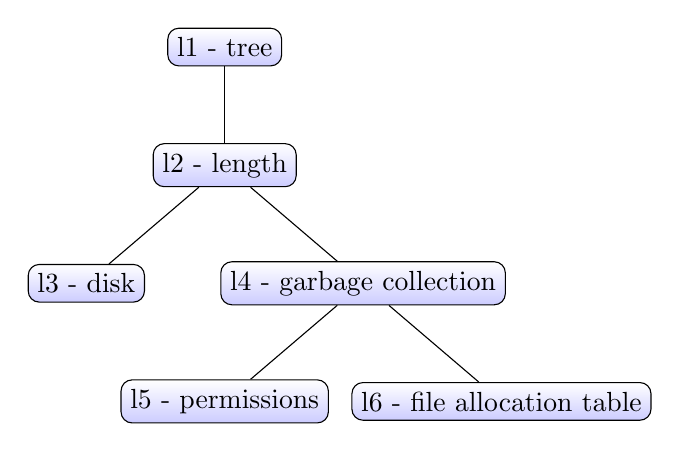
\begin{tikzpicture}[sibling distance=10em,
      every node/.style = {shape=rectangle, rounded corners,
        draw, align=center,
        top color=white, bottom color=blue!20}]
    \node {l1 - tree}
    child { node {l2 - length}
      child { node {l3 - disk}}
      child { node {l4 - garbage collection}
        child { node {l5 - permissions}}
        child { node {l6 - file allocation table}}}};
  \end{tikzpicture}
\end{figure}

At this point in development, we have six models of the filesystem,
here referred to as \texttt{l1} through \texttt{l6} (see
table \ref{model-description-table}). Each new model
\textit{refines} a previous model, adding some features and
complexity, and thereby approaching closer to a model which is binary
compatible with FAT32. These refinement relationships are shown in
figure \ref{refinement-figure}. \texttt{l0} is the simplest of these,
representing the filesystem as a literal tree; later models feature
file metadata (including ownership and permissions), externalisation
of file contents, and allocation/file allocation using an allocation
vector after the fashion of the CP/M file system.

Broadly, we characterise the filesystem
operations we offer as either \textit{write} operations, which do
modify the filesystem, or \textit{read} operations, which do not. In
each model, we have been able to prove \textit{read-over-write}
properties which show that write operations have
their effects made available immediately for reads at the same
location, but also that they do not affect reads at other locations.

The first read-after-write theorem states that immediately following a
write of some text at some location, a read of the same length at the
same location yields the same text. The second read-after-write
theorem states that after a write of some text at some location, a
read at any other location returns exactly what it would have returned
before the write. As an example, listings for the \texttt{l1} versions
of these theorems follow.

\medskip

\noindent
\begin{verbatim}
(defthm l1-read-after-write-1
  (implies (and (l1-fs-p fs)
                (stringp text)
                (symbol-listp hns)
                (natp start)
                (equal n (length text))
                (stringp (l1-stat hns fs)))
           (equal (l1-rdchs hns (l1-wrchs hns fs start text) start n) text)))

(defthm l1-read-after-write-2
  (implies (and (l1-fs-p fs)
                (stringp text2)
                (symbol-listp hns1)
                (symbol-listp hns2)
                (not (equal hns1 hns2))
                (natp start1)
                (natp start2)
                (natp n1)
                (stringp (l1-stat hns1 fs)))
           (equal (l1-rdchs hns1 (l1-wrchs hns2 fs start2 text2) start1 n1)
                  (l1-rdchs hns1 fs start1 n1))))
\end{verbatim}

By composing these properties, we can reason about executions
involving multiple reads and writes, as shown in the following
throwaway lemma.

\medskip

\noindent
\begin{verbatim}
(thm
 (implies (and (l1-fs-p fs)
               (stringp text1)
               (stringp text2)
               (symbol-listp hns1)
               (symbol-listp hns2)
               (not (equal hns1 hns2))
               (natp start1)
               (natp start2)
               (stringp (l1-stat hns1 fs))
               (equal n1 (length text1)))
          (equal (l1-rdchs hns1
                           (l1-wrchs hns2 (l1-wrchs hns1 fs start1 text1)
                                     start2 text2)
                           start1 n1)
                 (l1-rdchs hns1 (l1-wrchs hns1 fs start1 text1)
                           start1 n1))))
\end{verbatim}

\section{Proof methodology}

In \textit{l1}, our simplest model, the read-over-write properties
were, of necessity, proven from scratch, with the use of some rather
complicated induction schemes. For reference, the following code listing shows
the induction scheme used for \texttt{l1-read-after-write-2}.

\medskip

\noindent
\begin{verbatim}
(defun induction-scheme (hns1 hns2 fs)
  (if (atom hns1)
      fs
    (if (atom fs)
        nil
      (let ((sd (assoc (car hns2) fs)))
        (if (atom sd)
            fs
          (if (atom hns2)
              fs
            (if (not (equal (car hns1) (car hns2)))
                fs
              (let ((contents (cdr sd)))
                (if (atom (cdr hns1))
                    (cons (cons (car sd)
                                contents)
                          (delete-assoc (car hns2) fs))
                  (cons (cons (car sd)
                              (induction-scheme (cdr hns1) (cdr hns2) contents))
                                (delete-assoc (car hns2) fs)))))))))))
\end{verbatim}

In each subsequent model, the read-over-write properties are proven as
corollaries of equivalence proofs which establish the correctness of
read and write operations in the respective model with respect to a
previous model. A representation of such an equivalence proof can be
seen in figures \ref{l2-wrchs-correctness-1},
\ref{l2-rdchs-correctness-1} and \ref{l2-read-over-write-1}, which
respectively show the equivalence proof for \texttt{l2-wrchs}, the
equivalence proof for \texttt{l2-rdchs} and the composition of these
to obtain the first read-over-write theorem for model \texttt{l2}.


\begin{figure}
  \centering
  \caption{l2-wrchs-correctness-1}
  \label{l2-wrchs-correctness-1}
  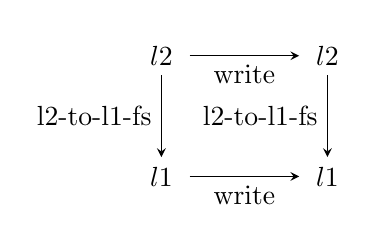
\begin{tikzpicture}
    \matrix (m) [matrix of math nodes,row sep=3em,column sep=4em,minimum width=2em]
            {
              l2 & l2 \\
              l1 & l1 \\};
            \path[-stealth]
            (m-1-1) edge node [left] {l2-to-l1-fs} (m-2-1)
            edge node [below] {write} (m-1-2)
            (m-2-1.east|-m-2-2) edge node [below] {write} (m-2-2)
            (m-1-2) edge node [left] {l2-to-l1-fs} (m-2-2);
  \end{tikzpicture}
\end{figure}

\begin{figure}
  \centering
  \caption{l2-rdchs-correctness-1}
  \label{l2-rdchs-correctness-1}
  \begin{tikzpicture}
    \matrix (m) [matrix of math nodes,row sep=3em,column sep=4em,minimum width=2em]
            {
              l2 & text \\
              l1 \\};
            \path[-stealth]
            (m-1-1) edge node [left] {l2-to-l1-fs} (m-2-1)
            edge node [below] {read} (m-1-2)
            (m-2-1.east|-m-2-2) edge node [below] {read} (m-1-2);
  \end{tikzpicture}
\end{figure}

\begin{figure}
  \centering
  \caption{l2-read-over-write-1}
  \label{l2-read-over-write-1}
  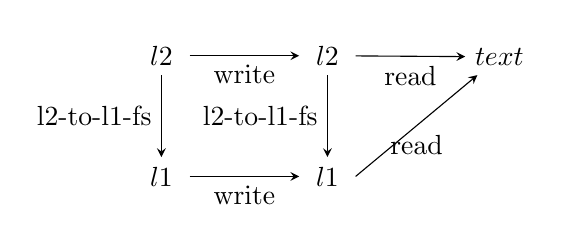
\begin{tikzpicture}
    \matrix (m) [matrix of math nodes,row sep=3em,column sep=4em,minimum width=2em]
            {
              l2 & l2 & text \\
              l1 & l1 \\};
            \path[-stealth]
            (m-1-1) edge node [left] {l2-to-l1-fs} (m-2-1)
            edge node [below] {write} (m-1-2)
            (m-2-1.east|-m-2-2) edge node [below] {write} (m-2-2)
            (m-1-2) edge node [left] {l2-to-l1-fs} (m-2-2)
            edge node [below] {read} (m-1-3)
            (m-2-2.east) edge node [below] {read} (m-1-3);
  \end{tikzpicture}
\end{figure}

\section{Some proof details}

As the models grow more complex, with the addition of more auxiliary
data the "sanity" criteria for filesystem instances become more
complex. For instance, in \texttt{l4}, the predicate \texttt{l4-fs-p}
is defined to be the same as \texttt{l3-fs-p}, which recursively
defines the shape of a valid filesystem. However, a "sane" filesystem
requires also that each disk index assigned to a regular file be
marked as \textit{used} in the allocation vector, and that it be
distinct from other disk indices assigned to files across the
filesystem. These properties are invariants to be maintained across
write operations; they simplify the verification of read-after-write
properties by ensuring that write properties do not create an
"aliasing" situation in which a regular file's contents can be
modified through a write to a different regular file.

These properties, in the form of the predicates
\texttt{indices-marked-listp} and \texttt{no-duplicatesp}, are
packaged together into the \texttt{l4-stricter-fs-p} predicate, for
which a listing follows.%%  It is interesting to note that disabling this
%% function brings down the compilation time for l4 from 20 seconds to and the
%% that for l6 from 84 seconds to .
It is interesting to note that disabling l6-wrchs brings down the
certification time for \texttt{l6} from 84 seconds to 64 seconds.

\medskip

\noindent
\begin{verbatim}
(defun l4-stricter-fs-p (fs alv)
  (declare (xargs :guard t))
  (and (l4-fs-p fs)
       (boolean-listp alv)
       (let ((all-indices (l4-list-all-indices fs)))
            (and (no-duplicatesp all-indices)
                 (indices-marked-p all-indices alv)))))
\end{verbatim}

\subsection{Citations}

For citations in the text please use
square brackets and consecutive numbers: \cite{jour}, \cite{lncschap},
\cite{proceeding1} -- provided automatically
by \LaTeX 's \verb|\cite| \dots\verb|\bibitem| mechanism.

\subsection{Page Numbering and Running Heads}

There is no need to include page numbers. If your paper title is too
long to serve as a running head, it will be shortened. Your suggestion
as to how to shorten it would be most welcome.

\section{LNCS Online}

The online version of the volume will be available in LNCS Online.
Members of institutes subscribing to the Lecture Notes in Computer
Science series have access to all the pdfs of all the online
publications. Non-subscribers can only read as far as the abstracts. If
they try to go beyond this point, they are automatically asked, whether
they would like to order the pdf, and are given instructions as to how
to do so.

Please note that, if your email address is given in your paper,
it will also be included in the meta data of the online version.

\section{BibTeX Entries}

The correct BibTeX entries for the Lecture Notes in Computer Science
volumes can be found at the following Website shortly after the
publication of the book:
\url{http://www.informatik.uni-trier.de/~ley/db/journals/lncs.html}

\subsubsection*{Acknowledgments.} The heading should be treated as a
subsubsection heading and should not be assigned a number.

\section{References}\label{references}

\bibliographystyle{splncs}
\bibliography{references}

\section*{Appendix: Springer-Author Discount}

LNCS authors are entitled to a 33.3\% discount off all Springer
publications. Before placing an order, the author should send an email, 
giving full details of his or her Springer publication,
to \url{orders-HD-individuals@springer.com} to obtain a so-called token. This token is a
number, which must be entered when placing an order via the Internet, in
order to obtain the discount.

\section{Checklist of Items to be Sent to Volume Editors}
Here is a checklist of everything the volume editor requires from you:


\begin{itemize}
\settowidth{\leftmargin}{{\Large$\square$}}\advance\leftmargin\labelsep
\itemsep8pt\relax
\renewcommand\labelitemi{{\lower1.5pt\hbox{\Large$\square$}}}

\item The final \LaTeX{} source files
\item A final PDF file
\item A copyright form, signed by one author on behalf of all of the
authors of the paper.
\item A readme giving the name and email address of the
corresponding author.
\end{itemize}
\end{document}
